\documentclass[fontsize=12pt,a4paper]{scrartcl}
\usepackage[utf8]{inputenc}
\usepackage{ragged2e}
\usepackage{mathtools}
\usepackage{setspace}

\usepackage{wrapfig}
% Example:
% \begin{wrapfigure}{R}{0.4\textwidth}
% \centering
% 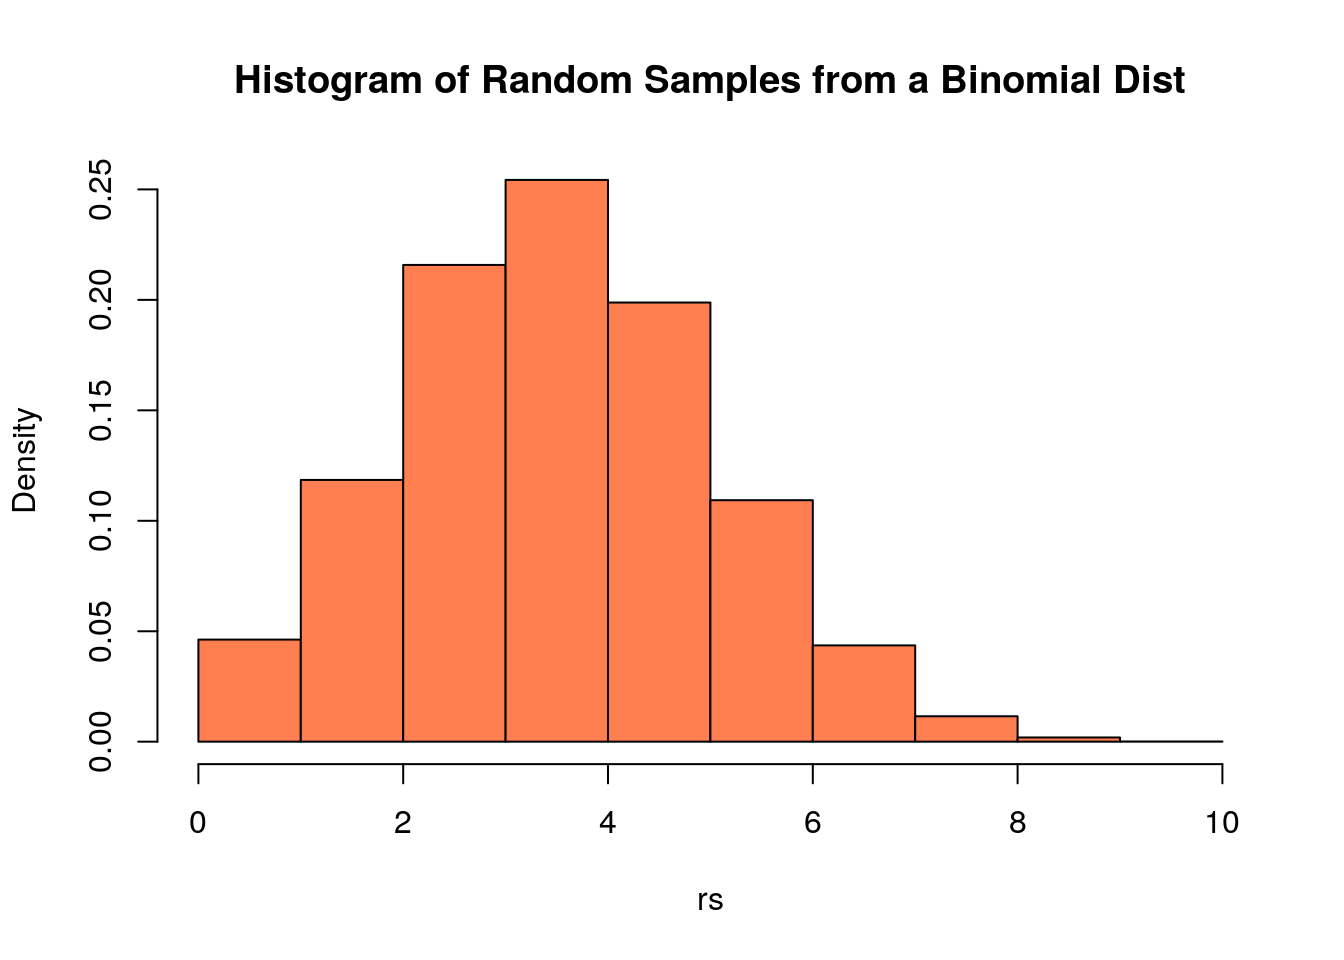
\includegraphics[width=0.35\textwidth]{assets/lectures_part_3-91d0349d.png}
% The PDF of the Student distribution.
% \end{wrapfigure}

\setlength{\parindent}{4em}
\setlength{\parskip}{1em}
\renewcommand{\baselinestretch}{1.4}


% \usepackage{esint}
\usepackage[english,russian, ukrainian]{babel}
\usepackage{misccorr,color,ragged2e,amsfonts,amsthm,graphicx,systeme,amsmath,mdframed,lipsum}
\renewcommand\qedsymbol{$\blacksquare$}
\renewcommand*{\proofname}{\text{Доведення}}
\theoremstyle{definition}
\newtheorem*{defo}{Означення}
\newtheorem*{teo}{Теорема}
\newtheorem*{example}{Приклад}
\theoremstyle{remark}
\newtheorem*{remark}{Зауваження}
\theoremstyle{definition}
\newtheorem*{consequence}{Наслідок}
\theoremstyle{definition}
\newtheorem{statement}{Утверждение}[section]
\newmdtheoremenv{boxteo}{Теорема}[section]
\setlength\parindent{0pt}
\DeclareMathOperator*\lowlim{\underline{lim}}
\DeclareMathOperator*\uplim{\overline{lim}}
\newcommand\independent{\protect\mathpalette{\protect\independenT}{\perp}}
\def\independenT#1#2{\mathrel{\rlap{$#1#2$}\mkern2mu{#1#2}}}
\usepackage{tikz}
\newcommand*\circled[1]{\tikz[baseline=(char.base)]{
  \node[shape=circle,draw,inner sep=1pt] (char) {#1};}}
\def\index#1{\mathbb{I}_{#1}}
\def\index{\mathbb{I}}
%
% \makeatletter
% %% make esint definition in line with amsmath
% \@for\next:={int,iint,iiint,iiiint,dotsint,oint,oiint,sqint,sqiint,
%   ointctrclockwise,ointclockwise,varointclockwise,varointctrclockwise,
%   fint,varoiint,landupint,landdownint}\do{%
%     \expandafter\edef\csname\next\endcsname{%
%       \noexpand\DOTSI
%       \expandafter\noexpand\csname\next op\endcsname
%       \noexpand\ilimits@
%     }%
%   }
% \makeatother
% Default fixed font does not support bold face
\DeclareFixedFont{\ttb}{T1}{txtt}{bx}{n}{12} % for bold
\DeclareFixedFont{\ttm}{T1}{txtt}{m}{n}{12}  % for normal

% Custom colors
\usepackage{color}
\definecolor{deepblue}{rgb}{0,0,0.5}
\definecolor{deepred}{rgb}{0.6,0,0}
\definecolor{deepgreen}{rgb}{0,0.5,0}

\usepackage{listings}

% Python style for highlighting
\newcommand\pythonstyle{\lstset{
language=Python,
basicstyle=\ttm,
otherkeywords={self},             % Add keywords here
keywordstyle=\ttb\color{deepblue},
emph={MyClass,__init__},          % Custom highlighting
emphstyle=\ttb\color{deepred},    % Custom highlighting style
stringstyle=\color{deepgreen},
frame=tb,                         % Any extra options here
showstringspaces=false            %
}}

\definecolor{javared}{rgb}{0.6,0,0} % for strings
\definecolor{javagreen}{rgb}{0.25,0.5,0.35} % comments
\definecolor{javapurple}{rgb}{0.5,0,0.35} % keywords
\definecolor{javadocblue}{rgb}{0.25,0.35,0.75} % javadoc

\lstset{language=C++,
basicstyle=\ttfamily,
keywordstyle=\color{javapurple}\bfseries,
stringstyle=\color{javared},
commentstyle=\color{javagreen},
morecomment=[s][\color{javadocblue}]{/**}{*/},
numbers=left,
numberstyle=\tiny\color{black},
stepnumber=2,
numbersep=10pt,
tabsize=4,
showspaces=false,
showstringspaces=false}


% Python environment
\lstnewenvironment{python}[1][]
{
\pythonstyle
\lstset{#1}
}
{}

% Python for external files
\newcommand\pythonexternal[2][]{{
\pythonstyle
\lstinputlisting[#1]{#2}}}

% Python for inline
\newcommand\pythoninline[1]{{\pythonstyle\lstinline!#1!}}
%
% \begin{python}
% class MyClass(Yourclass):
%     def __init__(self, my, yours):
%         bla = '5 1 2 3 4'
%         print bla
% \end{python}

\begin{document}



\def\be{\begin{equation}}      % equation
\def\ee{\end{equation}}        % ...
\def\bd{\begin{defo}}          % definition
\def\ed{\end{defo}}            % ...
\def\bbt{\begin{boxteo}}       % boxteo
\def\ebt{\end{boxteo}}         % ...
\def\i{\infty}                 % infty
\def\d{\partial}               % dx dy - partial     = \d
% \def\ind{\mathbb{I}_}          % indicator           = \ind
\def\xx{\chi_{\overline{\xi}}} % char of vec xi = \xx
\def\Laplas{\text{Ф}}          % Laplas function     = \Laplas
\def\veta{\overline{\eta}}     % vector eta          = \veta
\def\vxi{\overline{\xi}}       % vector xi           = \vxi
\def\vtheta{\overline{\theta}} % vector theta   = \vtheta
\def\gammadistr{\Gamma}
\def\bdash{\ \Big|\  }


\tableofcontents

\newpage
\def\red#1{\textbf{\color{javared}#1}}
\def\blue#1{\textbf{\color{javadocblue}#1}}
\def\card{\text{card}}

\begin{center}
	\Huge \textbf{Собственно, матстат...}
\end{center}
\section{Описова статистика.}
\subsection{Основнi поняття математичної статистики.}
 \begin{itemize}
 \item\textbf{\color{javared} Математична статистика} -- це розділ математики, в якому вивчаються методи збору, систематизації та обробки інформації з метою виявлення існуючих закономірностей.
   \end{itemize}
     У математичній статистиці набір даних розглядається як реализація або спостереження деякої випадкової величини (в.в.) $\xi$, яка визначена на деякому ймовірнісному просторі $\left( \Sigma, \mathcal{F}, P \right)$, пов'язаний із стохастичним експериментом.
   \begin{itemize}
     \item \textbf{\color{javared} Генеральна сукупність} (population) --  це (як правило, невідомий) ймовірнісний розподіл $\mathcal{F}$ в.в. $\xi$, що спостерігається (ймовірнісна міра $P$)
     \item \textbf{\color{javared} Вибірка} (sample) -- це набір незалежних в.в. $\xi_1, \xi_2 ,..., \xi_n$, кожна з яких має розподіл $\mathcal{F}$. При цьому $n$ називається об'ємом вибірки.
     \item \textbf{\color{javared} Реалізація вибірки} -- це значення $x_1 , x_2 , ... , x_n$ або $\overrightarrow{x} = \begin{bmatrix}
      x_1 & \cdots & x_n
     \end{bmatrix}$, які прийняли в.в. $\xi_1 , ... , \xi_n$ в результаті конкретного стохастичного експерименту. При цьому $x_k$ називається \textbf{\color{javadocblue} варiантою}. Тобто:
     $$
     \begin{gathered}
      \left( \Sigma , \mathcal{F}, P \right)\\
      \omega_o \in \Sigma
     \end{gathered} \qquad x_1 = \xi_1(\omega_0)\ , \ \cdots \ , \  x_n  = \xi_n (\omega_0) \qquad \begin{array}{r}
      \text{Вибірка: } (\xi_1 , ..., \xi_n) \\
      \text{Реал. вибірки: } (x_1 , ... , x_n)
     \end{array}
     $$
 \end{itemize}
Основою будь-яких висновкiв щодо властивостей г.с. $\mathcal{F}$ є \textbf{\color{javadocblue} вибiрковий метод}, суть якого полягає в тому, що властивостi в.в. $\xi$
визначаються шляхом вивчення цих властивостей
на випадковiй вибiрцi. Множина всiх реалiзацiй $S$ вибiрки $x_1 , \dots , x_n$ називається \textbf{\color{javadocblue} вибiрковим простором}.

\begin{itemize}
\item Пара $(S,\mathcal{F})$ називається \textbf{\color{javadocblue} статистичною моделлю} опису серiї спостережень, якi породжують вибiрку. \item Якщо розподiл $\mathcal{F}_{\xi}$ вiдомий з точнiстю до невiдомого вектора параметрiв $\overrightarrow{\theta} = \begin{bmatrix}
 \theta_1 & \cdots & \theta_q
\end{bmatrix}$ з множиною значень
$\Theta (\overrightarrow{\theta} \in \Theta)$
, тодi статистичну модель називають \textbf{\color{javadocblue} параметричною моделлю},
а множину $\Theta$ - параметричною множиною.
\item \textbf{\color{javared} Статистикою} (або вибiрковою характеристикою) називається довiльна борелева функцiя $g(\overrightarrow{\xi}) = g(\xi_1, \dots , \xi_n)$ вiд елементiв вибiрки. Розподiл цiєї в.в. називається
\textbf{\color{javadocblue} вибiрковим розподiлом}, а значення $g(\overrightarrow{x})$  статистики за реалiзацiєю $\overrightarrow{x}$ - \textbf{ \color{javadocblue} вибiрковим
значенням}.
\end{itemize}
Статистичну модель називають неперервною або дискретною, якщо розподiл г.с. $\mathcal{F}_\xi$ є
неперервним або дискретним.
\begin{itemize}
\item
\textbf{\color{javared} Описова статистика} (або дескриптивна статистика, англ. descriptive statistics) – це
роздiл статистики, що займається обробкою емпiричних даних, їх систематизацiєю та
наочним представленням у виглядi графiкiв та таблиць.
\item
\textbf{\color{javared} Cтатистичнi виводи} (англ. inferential statistics) – це роздiл статистики, що займається
вивченням зв’язкiв мiж вибiрковими даними та г.с., з яких вона отримана.
\end{itemize}
Зокрема, статистичнi виводи займаються вiдповiддю на питання, якi висновки можна зробити
щодо г.с. (функцiя розподiлу, щiльнiсть або закон розподiлу, числовi характеристики такi як
математичне сподiвання, дисперсiя, моменти в.в., тощо) за вибiркою.
\subsection{Типи даних.}
\begin{center}
 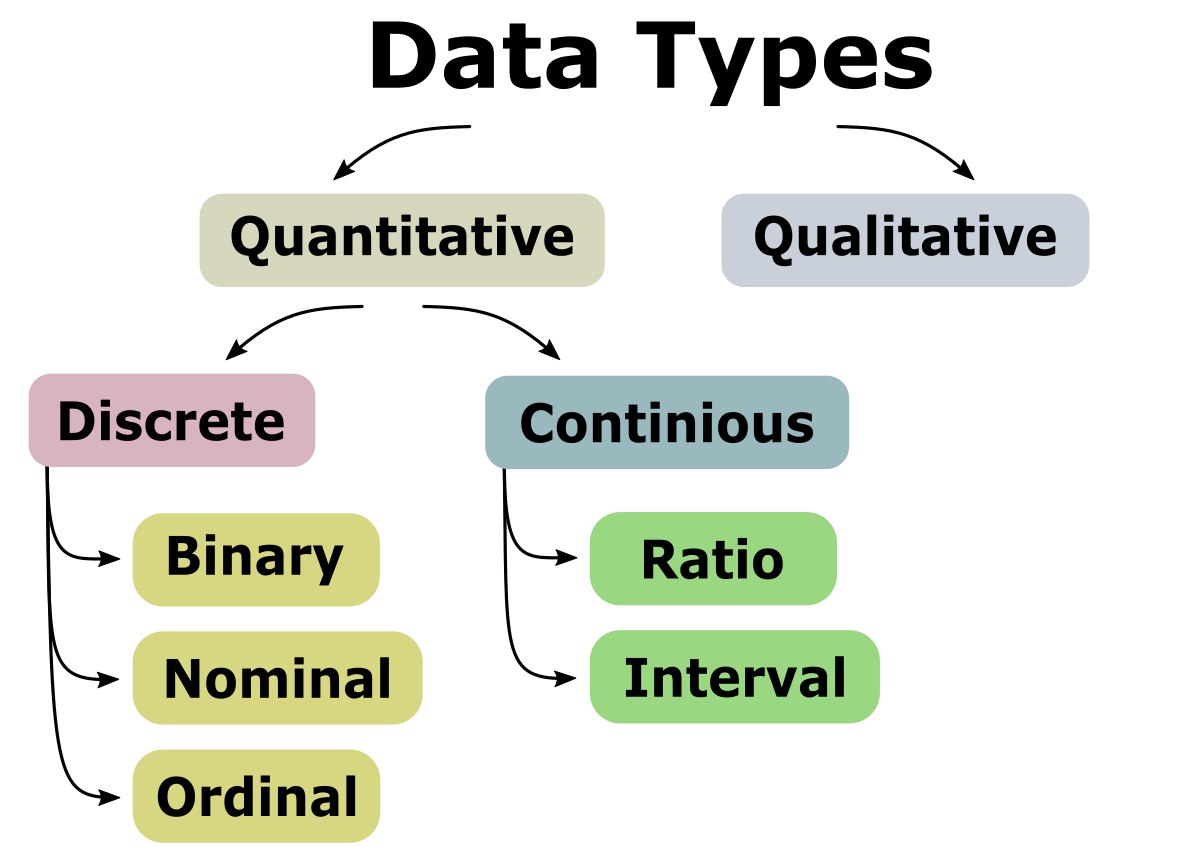
\includegraphics[scale=0.36]{assets/lectures_part_5-a3868f99.png}
\end{center}
\begin{itemize}
    \item \textbf{\color{javared} Кiлькiснi данi } використовують чисельнi значення для опису об’єкта, що нас цiкавить.
    \begin{itemize}
        \item \textbf{\color{javadocblue}Дискретнi данi} вiдповiдають вибiрцi з дискретного розподiлу г.с.
Дискретнi данi зазвичай є цiлими числами, хоча можуть задаватись i десятковими
дробими. Їх особливiстю є те, що вони мають ”пробiли” (”дiри”) у своїх можливих
значеннях.
\item
\textbf{\color{javadocblue}Неперервнi данi} вiдповiдають вибiрцi з неперервного розподiлу г.с.
Неперервнi данi приймають будь-якi значення з певного дiапазону i не мають
стрибкiв
    \end{itemize}
\item \textbf{\color{javared}Якiснi данi} використовують описовi вирази для вимiрювання або класифiкацiї об’єкта,
що нас цiкавить.
\end{itemize}
\newpage
\subsection{Первинна обробка інформації.}
\begin{itemize}
    \item \textbf{\color{javared}Варіаційним рядом} $x_{(1)} \leq x_{(2)} \leq \cdots \leq x_{(n)} $ називаються елементи вибiрки, якi
впорядкованi за зростанням. При цьому:
$$
x_{(1)} = \min\limits_{1 \leq k \leq n} x_k \qquad \quad x_{(n)} = \max\limits_{1 \leq k \leq n} x_k
$$
$x_k$ називається \textbf{\color{javadocblue}порядковою статистикою порядку k}.
\end{itemize}
Процес впорядкування вибiрки називається \textbf{\color{javadocblue}''ранжуванням''}.\par
\red{Розмах вибiрки} $R$ --- рiзниця мiж найбiльшим та найменшим елементами, тобто:
$$
R = x_{(n)} - x_{(1)}
$$
Нехай розподіл г.с. $\mathcal{F}$ є дискретним. Тодi нехай $x_1^* , \dots , x_m^*$ – елементи вибiрки, впорядкованi
за зростанням, причому кожне значення вказується лише один раз, $n_k$ – число разiв появи $x_k^*$ в реалiзацiї вибiрки.  $n_k$ називається \red{частотою} появи $x_k^*$.\par
Зауважимо, що $n_1 + \dots + n_m = n$.\par
Сума частот елементiв $ \displaystyle\sum\limits_{i = 1}^{ \textbf{k}}{x_i^*}$ називається \blue{кумулятивною частотою} $n_k^*$:
$$
n_k^* = n_1 + ... + n_k
$$
Величина $\nu_k = \dfrac{n_k}{n}$ називається \red{вiдносною частотою}.\par
Сума вiдносних частот елементiв $\displaystyle  \sum\limits_{i = 1}^{k}{ \nu_i}$ називається \blue{кумулятивною
вiдносною частотою} елементу $x_k^*$.\par
\newpage
\begin{center}
\subsubsection{Статистичний ряд.}
На основі вказаних вище характеристик можна побудувати \red{статистичний ряд}:\par
\begin{tabular}{|c|c|c|c|c|}
\hline
\begin{tabular}[c]{@{}c@{}}Значення \\ $(x_k^*)$\end{tabular} & \begin{tabular}[c]{@{}c@{}}Частоти \\ $(n_k)$\end{tabular} & \begin{tabular}[c]{@{}c@{}}Кумулятивнi частоти \\ $(n_k^*)$\end{tabular} & \begin{tabular}[c]{@{}c@{}}Вiдноснi частоти \\ $(\nu_k)$\end{tabular} & \begin{tabular}[c]{@{}c@{}}Кумулятивнi вiдноснi\\ частоти $(\nu_k^*)$\end{tabular} \\ \hline
$x_1^*$ & $n_1$ & $n_1^*$ & $\nu_1=\frac{n_1}{n}$ & $\nu_1^*$ \\ \hline
$x_2^*$ & $n_2$ & $n_2^* = n_1 + n_2$ & $\nu_2=\frac{n_2}{n}$ & $\nu_2^*$ \\ \hline
$\vdots$ & $\vdots$ & $\vdots$ & $\vdots$ & $\vdots$ \\ \hline
$x_m^*$ & $n_m$ & $n_m^* = \sum\limits_{i=1}^m n_i = n$ & $\nu_m=\frac{n_m}{n}$ & $\nu_m^* = \sum\limits_{i=1}^m \nu_i = 1$ \\ \hline
\end{tabular}
\end{center}

Якщо розподiл г.с. є неперервною або дискретною з великою кiлькiстю значень, тодi використовують \red{iнтервальний статистичний ряд}.\par
Область, в якому лежать всi значення реалiзацiї вибiрки розбивають на \blue{m класiв}:
$$
\Delta_1 = [y_0, y_1) , \cdots , \Delta_m = [y_{m-1}, y_m]
$$
Кiлькiсть класiв зазвичай варiюється в межах 5 - 20. Інодi, для визначення кiлькостi класiв
використовують \blue{формулою Стреджеса}:
$$
m-1 = \log_2{n}
$$
\begin{remark}
Реалiзацiя вибiрки може мiстити так званi \red{викиди}. У випадку наявностi викiдiв або великої
порожнiх класiв на початку або в кiнцi вибiрки, доцiльно використовувати при розбитi
класи з вiдкритими кiнцями (клас, що має лише нижню або верхню межу).
\end{remark}

\begin{remark}
В деяких випадках спостереження можуть надаватись не як iндивiдуальнi значення, а вже
розподiленi по iнтервалах тобто у виглядi iнтервального статистичного розподiлу. В цьому
випадку данi називаються \red{групованими}.
\end{remark}
\newpage
\subsection{Графiчнi методи представлення iнформацiї.}

\begin{wrapfigure}[5]{R}{0.43\textwidth}
\vspace*{-2em}
\centering
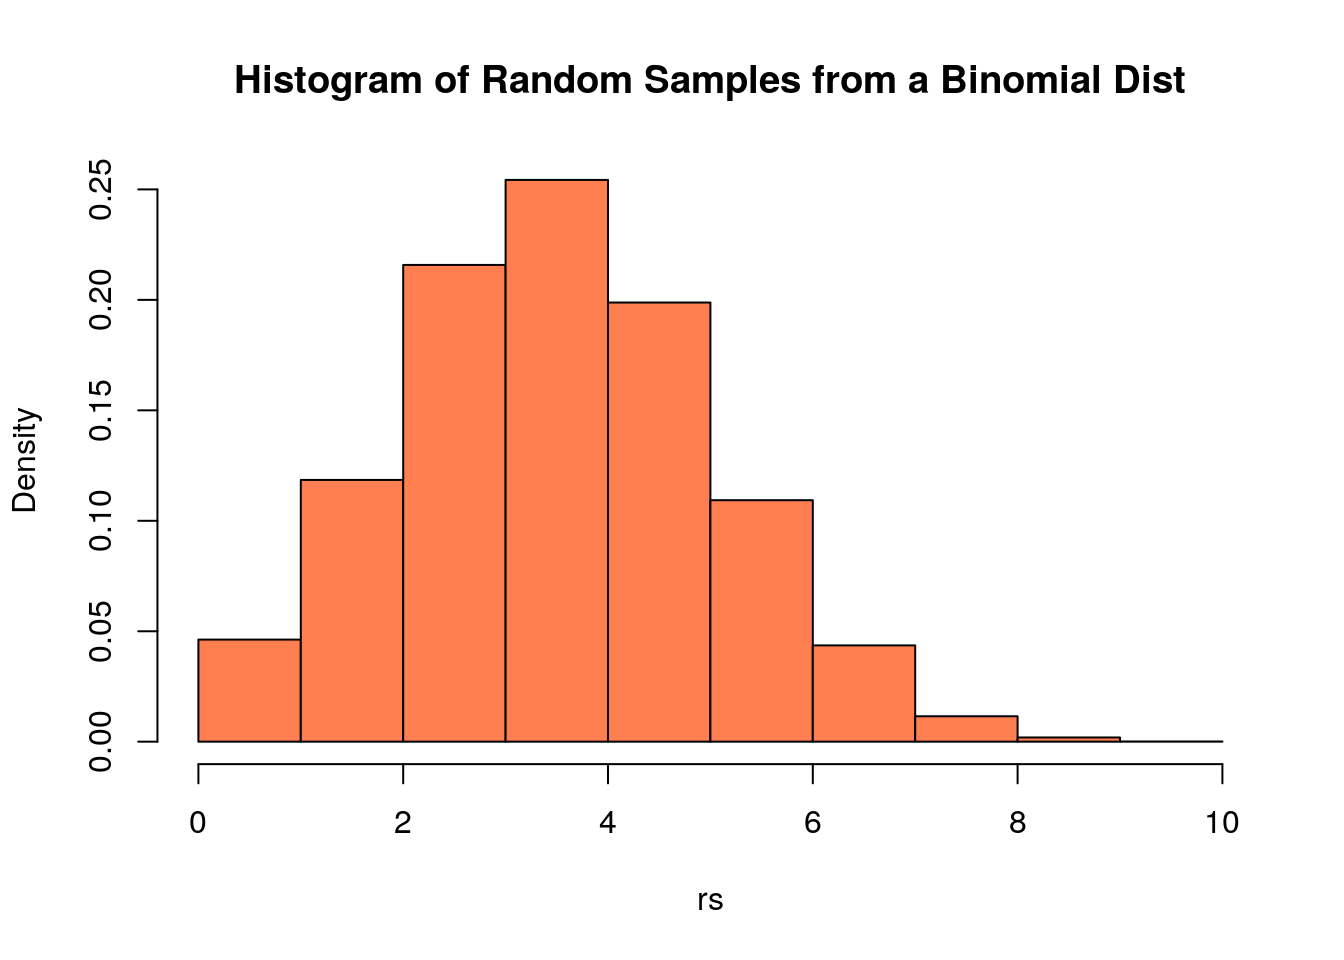
\includegraphics[width=0.41\textwidth]{assets/lectures_part_3-91d0349d.png}
\end{wrapfigure}

\subsubsection{Гiстограма.}

Якщо розподiл г.с. є неперервним, гiстограма будується на основi iнтервального статистичного розподiлу г.с. наступним чином: будують систему координат таку, що на осi
абсцис будуть вiдображатися iнтервали $\Delta_1 , ... , \Delta_m$, а на осi ординат вiдповiднi частоти. \par Далi будують у вказанiй системi координат прямокутники з основами $\Delta_k, k \in \overline{1,m}$,
та вiдповiдними висотами $n_k$.\par
Також використовують гiстограму вiдносних частот, в якiй висота стовпцiв
визначається за формулою:
$$
h_k = \frac{\nu_k}{l(\Delta_k)}
$$
Зауважимо, що в цьому випадку площа отриманої фiгури буде дорiвнювати 1.
\subsubsection{Полігон частот.}
\begin{wrapfigure}[10]{R}{0.43\textwidth}
\vspace*{-2em}
\centering
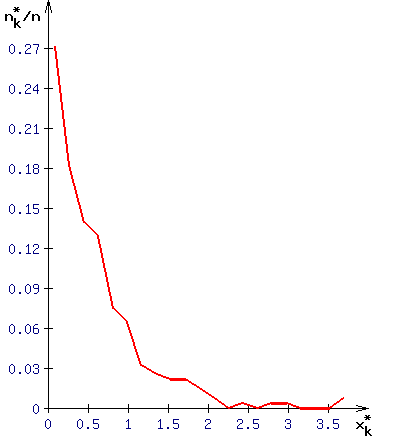
\includegraphics[width=0.41\textwidth]{assets/lectures_part_5-567b0078.png}
\end{wrapfigure}
Якщо розподiл г.с. є дискретним, тодi полiгон частот будується на основi статистичного
розподiлу г.с. наступним чином: будують систему координат таку, що на осi абсцис будуть вiдображатися елементи вибiрки $x_1^*, \dots , x_m^*$, а на осi ординат вiдповiднi частоти.\par Далi у вказанiй системi координат будують точки $M_k (x_k^*, n_k), k= \overline{1,m}$, якi з’єднують
мiж собою у ламану $M_1M_2\dots M_m$
\newpage
\section{Дискриптивні міри.}
Графiчнi методи є чудовим способом для отримання швидкого огляду вибiркових даних, але
вони не є точними та не призводять самi по собi до наступних дослiджень. Для цього нам
потрiбно введення числових параметрiв таких як, наприклад, середнє.\par
Iснують рiзнi шляхи, за допомогою яких ми можемо спробувати описати розподiл. Розглянемо
деякi з них, якi кориснi при описi гiстограми або полiгона частот.\par
Надалі, нехай $x_1, \dots, x_n$ реалiзацiя вибiрки з г.с. $\mathcal{F}$.

\subsection{Мiри центральної тенденцiї (measures of central tendency).}
\subsubsection{Вибiркове середнє.}
Вибiркове середнє $\overline{x}$ є одним iз найбiльш вiдомих параметрiв центральної тенденцiї i знаходиться за формулою:
$$
\overline{x} = \frac{1}{n}  \sum\limits_{k =1 }^{n}{x_k}
$$
\begin{remark}
    Вказана формула може бути використана лише у випадку, коли всi iндивiдуальнi значення $x_j$ є вiдомими.
\end{remark}
Якщо ж вiдносно вибiрки є вiдомим лише розбиття спостережень на класи $(\Delta_i)$ та частота
попадань елементiв вибiрки у кожен з цих iнтервалiв $(n_i)$. В цьому випадку групованих даних
можна використовувати наступну формулу:
$$
\overline{x} = \frac{1}{n}  \sum\limits_{i = 1}^{m}{n_i x_i^*} = \sum\limits_{i = 1}^{ m}{\nu_i x_i^*}
$$
\subsubsection{Вибiркова медiана.}
Однiєю iз вад вибiркового середнього воно дає нерепрезентативнi результати, оскiльки є
чутливим до викидiв у вибiрцi та симетрiї. Тому iнодi є бiльш привабливим використання iнших параметрiв. Наприклад, \red{вибіркової медіани}.\par
Нехай у вибiрцi вiдомi всi iндивiдуальнi спостереження. Будуємо варiацiйних ряд:
$$
x_{(1)} \leq x_{(2)} \leq \cdots \leq x_{(n)}
$$
Знаходимо медіану як середнiй елемент цього варiацiйного ряду $M_e^*$:
$$
M_e^* = \begin{dcases}
 x_{(k+1)}, & n = 2k+1;\\
 \frac{x_{(k)} + x_{(k+1)}}{2}, & n =2k;
\end{dcases}
$$
Якщо вибiрка представлена групованими даними, тодi вибiркова медiана розраховується
наступним чином:
\begin{enumerate}
    \item Знаходимо клас (позначимо його номер $me$), що буде мiстити елемент, який вiдповiдає медiанi, тобто:
    $$
    n^*_{me-1} < \frac{n}{2} \qquad n^*_{me} \geq  \frac{n}{2}
    $$
    \item Елемент знайденого класу, що буде вiдповiдати медiанi, обчислюємо за наступною формулою:
    $$
    M_e^* = y_{me-1} + (y_{me} - y_{me-1})    \frac{ \frac{n}{2} - n_{me}^* -1 }{n_{me}}
    $$
\end{enumerate}
Зазначимо, що дрiб у правiй частинi останньої рiвностi вказує нам, яку частину iнтервалу
ми маємо пройти, щоб дiйти до медiани.
\subsubsection{Вибiркова мода.}
\red{Вибiркова мода} $M_o^*$ --- це елемент вибiрки, який зустрiчається частiше за все.\par

У випадку групованих даних визначення бiльш складне. Клас (позначимо його номер $mo$), який має найбiльшу частоту, називається \blue{модальним}, причому при розбитi на iнтервали, вони
мають бути однакової ширини.\par
Значення моди знаходиться за формулою:
$$
M_{o}^* y_{mo-1} + (y_{mo} - y_{mo-1}) \frac{n_{mo} - n_{mo-1}}{(n_{mo} - n_{mo-1}) + (n_{mo} - n_{mo+1})}
$$
\begin{remark}
Вказанi три параметри центральної тенденцiї дають рiзну iнформацiю. Але якщо розподiл
симетричний, то вони будуть давати приблизно однаковi значення.
\end{remark}
\newpage
\subsection{Мiри розсiювання (Measure of dispersion)}
При розгядi двох рiзних розподiлiв, вони можуть мати однаковi або дуже близькi середнi, але
при цьому суттєво вiдрiзнятись. Наприклад, при порiвняннi рiвня добробуту двох країн: у них
може бути дуже близькими середнiй добробут по країнi, але в однiй країнi всi отримують
приблизно однаковий рiвень достатку, а в iнший можуть екстремальнi значення великого
достатку та злиденного. Параметри розсiювання як раз i потрiбнi для вiдокремлення таких
випадкiв.
\subsubsection{Розмах вибiрки (range).}
Розмах вибiрки є найпростiшою мiрою розсiювання, який обчислюється як рiзниця мiж найбiльшим та найменшим спостереженням даної вибiрки:
$$
R = x_{(n)} - x_{(1)}
$$
\subsubsection{Середнє абсолютне вiдхилення (mean absolute error).}
Якщо вiдомо математичне сподiвання розподiлу $\mathcal{F}, \mathbb{E} \xi_j = \mu$ , тодi cереднє абсолютне вiдхилення розраховується наступним чином:

\begin{itemize}
    \item Якщо данi не групованi, то:
    $$
    MAE = \frac{1}{n}  \sum\limits_{j = 1}^{n}{\left| x_j - \mu \right|}
    $$
    \item Якщо данi групованi, то:
    $$
    MAE = \frac{1}{n}  \sum\limits_{j = 1}^{m}{n_i \left| x^*_j - \mu \right|} =  \sum\limits_{j =1 }^{m}{ \nu_j \left| x_j^* - \mu \right|}
    $$
\end{itemize}
Якщо ж математичне сподiвання не вiдомо, то $\mu$ у формулах змінюється на $\overline{x}$.
\subsubsection{Вибiркова дисперсiя (variance).}
Найбiльш корисним параметром розсiювання є \red{вибiркова дисперсiя}. Вона є середнiм квадратiв вiдхилень елементiв вибiрки вiд середнього значення.\par
Якщо $ \mathbb{E} \xi_j = \mu$, тодi вибiркова дисперсiя розраховується наступним чином:
\begin{spacing}{1}
\begin{enumerate}
    \item Якщо данi не групованi, то:
    $$
    \sigma_*^2 = \mathbb{D}^*_{\xi} = \frac{1}{n}  \sum\limits_{j = 1}^{n}{
    (x_j - \mu)^2
    }
    $$
    \item Якщо данi групованi, то:
    $$
    \sigma_*^2 = \mathbb{D}^*_{\xi} = \frac{1}{n}  \sum\limits_{i = 1}^{m}{n_i (x_i^* - \mu)^2}
    $$
\end{enumerate}
Якщо ж $\mathbb{E}\xi_j$ не вiдомо, тодi розглядають або \blue{вибiркову
дисперсiю}.
\vspace*{-0.5em}
\begin{enumerate}
    \item Якщо данi не групованi, то:
    $$
    s^2 = \mathbb{D}^{**}_{\xi} = \frac{1}{n}  \sum\limits_{j = 1}^{n}{
    (x_j - \overline{x})^2
    }
    $$
    \item Якщо данi групованi, то:
    $$
    s^2 = \mathbb{D}^{**}_{\xi} = \frac{1}{n}  \sum\limits_{i = 1}^{m}{n_i (x_i^* - \overline{x})^2}
    $$
\end{enumerate}
\vspace*{-1em}
Або \blue{виправлену (незмiщену) вибiркову дисперсiю}.
\vspace*{-0.5em}
\begin{enumerate}
    \item Якщо данi не групованi, то:
    $$
    s^2_0 = \mathbb{D}^{***}_{\xi} = \frac{1}{n-1}  \sum\limits_{j = 1}^{n}{
    (x_j - \overline{x})^2
    }
    $$
    \item Якщо данi групованi, то:
    $$
    s^2_0 = \mathbb{D}^{***}_{\xi} = \frac{1}{n-1}  \sum\limits_{i = 1}^{m}{n_i (x_i^* - \overline{x})^2}
    $$
\end{enumerate}
\end{spacing}
\subsubsection{Стандартне вiдхилення (standard deviation).}
Оскiльки при знаходженнi дисперсiї ми підносимо вiдхилення до квадрату, то не зовсiм зрозумiлим є одиницi вимiрювання дисперсiї. Тому природньо взяти вiд цього виразу корiнь квадратний. \par

Таким чином, ми отримуємо величину, рiвну корню квадратному вiд вибiркової дисперсiї, яка називається \red{стандартним вiдхиленням} i задається виразом:
$$
\sigma_{\xi}^{*, **, ***} = \sqrt{\mathbb{D}_{\xi}^{*, **, ***}}
$$
\subsubsection{Коефiцiєнт варiацiї (coefficient of variation).}
\red{Коефiцiєнт варiацiї} (вiдносне стандартне вiдхилення) визначається, як процентне вiдношення стандартного вiдхилення до вибiркового середнього.
$$
C_V = \frac{s_0}{x} \cdot 100\%
$$
\begin{remark}
Вiн є вiдносним показником розсiювання(мiнливостi) ознаки(вибiрки) по вiдношенню до середнього показника вибiрки. (Може використовуватися лише для вiдносного рiвня вимiрювання).
Використання коефiцiєнта варiацiї є суттєвим лише при вивченнi ознаки, яка має \blue{додатне
значення}.
\end{remark}
\newpage
\subsection{Мiри позицiї.}
Мiри позицiї є iндикаторами, як окрема величина спiввiдноситься з iншими.
\subsubsection{Квантиль.}
  Нехай $\alpha \in (0,1)$. \red{$\alpha$-квантилем} в.в. $\xi$ називається
таке число $q_{\alpha} \in \mathbb{R}$, що:
$$
\mathbb{P} \left\lbrace \xi \leq q_{\alpha} \right\rbrace \geq \alpha \qquad \qquad \mathbb{P} \left\lbrace \xi\geq q_{\alpha} \right\rbrace \geq 1 - \alpha
$$
\begin{wrapfigure}{R}{0.5\textwidth}
\vspace*{-2em}
\centering
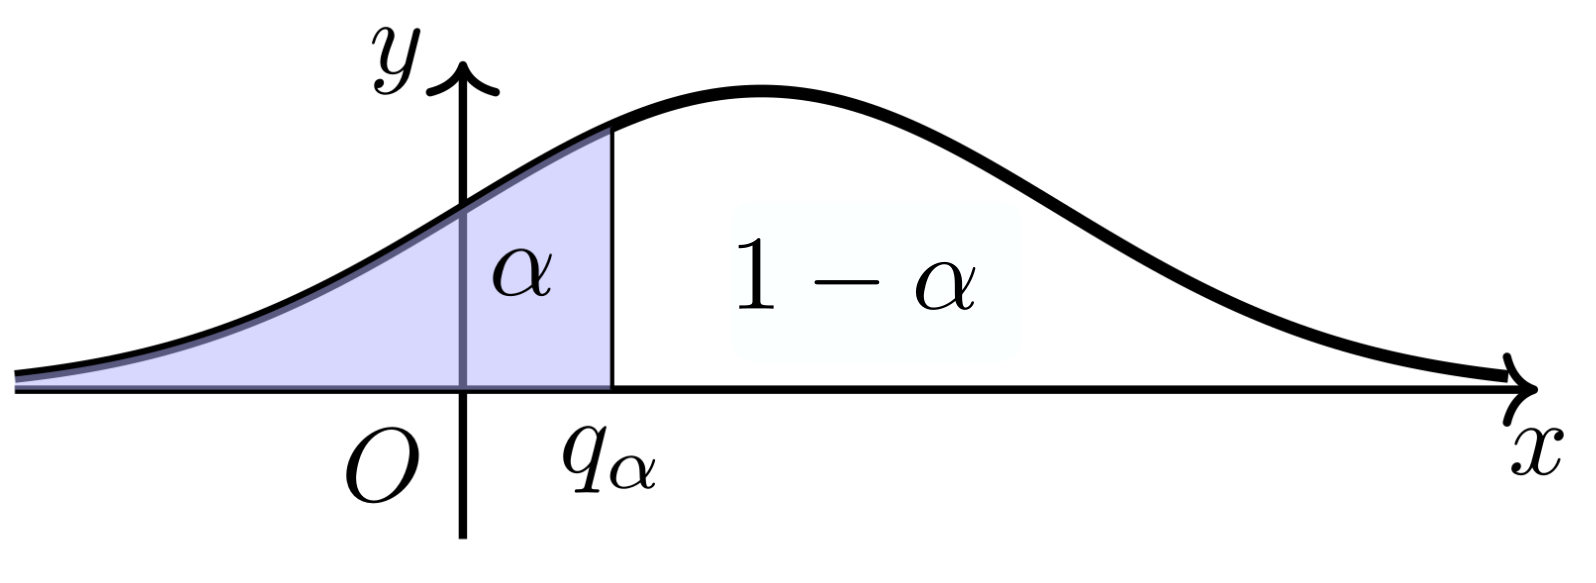
\includegraphics[width=0.48\textwidth]{assets/lectures_part_5-94f6ab31.png}
\end{wrapfigure}

Зауважимо, що для неперервних в.в. \\ $\alpha$-квантиль однозначно знаходиться з\\ рiвняння:
$$
F(q_{\alpha}) = \alpha
$$
де $F$ - функція розподілу в.в. $\xi$.\\
Знайдемо, як слiд шукати вибiрковi значення квантилiв. Якщо у вибiрцi вiдомi всi iндивiдуальнi спостереження. Побудуємо варiацiйних ряд:
$$
x_{(1)} \leq x_{(2)} \leq  \dots \leq x_{(n)}
$$
Елемент, що буде вiдповiдати $\alpha$-квантилю цього варiацiйного ряду:
$$
q_{\alpha} = \begin{dcases}
x_{( \left| K \right| + 1 )} , & K = n\cdot \alpha \notin \mathbb{Z};\\
\frac{x_{(K)} + x_{( K + 1 )}}{2} , & K = n\cdot \alpha \in \mathbb{Z};\\
\end{dcases}
$$
Для групованих даних $\alpha$-квантиль $q_{\alpha}$ визначається наступним чином:
\begin{enumerate}
    \item Знаходимо клас (позначимо його номер $K_{\alpha}$), що буде мiстити $\alpha$-квантиль, тобто:
    $$
    n_{K_{\alpha} -1}^* < n \cdot \alpha \qquad \quad n_{K_{\alpha}}^* \geq n \cdot \alpha
    $$
    де $n_i^*$ --- кумулятивна частота $i$-го класу;
    \item Обчислюємо значення $\alpha$-квантиля за наступною формулою:
    $$
    q_{\alpha} = y_{K_{\alpha} -1} + (y_{K_{\alpha}} - y_{K_{\alpha}-1}) \frac{\alpha \cdot n - n^*_{K_{\alpha}-1}}{n_{K_{\alpha}}}
    $$
    де $y_{K_{\alpha-1}}, y_{K_{\alpha}}$ --- вiдповiдно нижня та верхня межi класу, який мiстить квантиль, $n_{K_{\alpha}}$ --- частота класу, який мiстить квантиль.
\end{enumerate}
\subsubsection{Процентиль.}
\red{$p$-процентилем} (percentile) називається величина $P_p$, яка спiвпадає з квантилем порядку $\alpha = \dfrac{p}{100} $ тобто:
$$
P_p = q_{ \frac{p}{100} }
$$
\blue{Квартилями (quartile)} називають процентилi кратні 25-ти:
\begin{itemize}
    \item $Q_1 = P_{25}$ --- нижній квартиль;
    \item $Q_1 = P_{50} = M_e$ --- медіана;
    \item $Q_1 = P_{50} = M_e$ --- медіана;
\end{itemize}
\blue{Децилями (decile)} називають процентилi кратні 10-ти:
$$
D_1 = P_{10} , D_2 = P_{20} , \dots , D_9 = P_{90}
$$
\blue{Мiжквартильним дiапазоном (interquartile range)} називають величину:
$$
IQR = Q_3 - Q_1
$$
Помiтимо, що мiжквартильний дiапазон є мiрою розсiювання. Його недолiком є те, що вiн вимiрює розкид в серединi
даних, а не по всiй множинi.
\subsection{Мiри форми.}
Мiри форми – є iндикаторами симетричностi та ''згладженостi'' даних.
\subsubsection{Вибірковий момент.}
\red{Вибiрковим моментом} k-го порядку називається величина:
$$
\overline{x}^k = \frac{1}{n}  \sum\limits_{j = 1}^{n}{x_j^k}
$$
\blue{Вибiрковим центральним моментом} k-го порядку називається величина:
$$
\overline{\mu}_k = \frac{1}{n}  \sum\limits_{j = 1}^{n}{(x_j - \overline{x})^k}
$$

\subsubsection{Коефiцiєнт асиметрiї (skewness).}
\red{Коефiцiєнтом асиметрiї} називається число:
$$
A_S = \frac{\overline{\mu}_3}{s_0^3}
$$
\begin{center}
 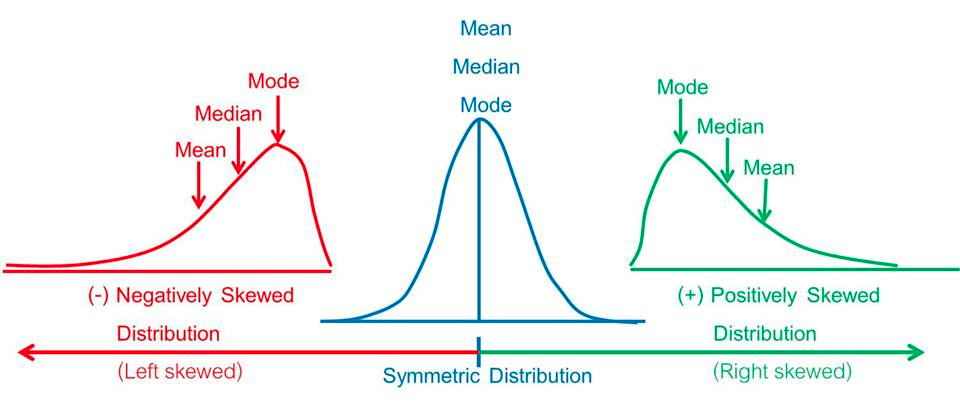
\includegraphics[scale=0.45]{assets/lectures_part_5-ad0b36c5.png}
\end{center}
Коефiцiєнтом асиметрiї характеризує \blue{мiру скошеностi розподiлу} даних щодо вибiркового середнього:
\begin{itemize}
\item $As = 0$ -- данi симетричнi щодо середнього;
\item $As > 0$ -- данi мають правосторонню асиметрiю;
\item $As < 0$ -- данi мають лiвосторонню асиметрiю.
\end{itemize}
\subsection{Коефiцiєнт асиметрiї Пiрсона.}
\red{Коефiцiєнтом асиметрiї Пiрсона} називається число:
$$
Sk = \frac{\overline{x} - M_0}{s_0}
$$
Недолiком коефiцiєнта асиметрiї Пiрсона полягає в тому, що вiн враховує лише центральну
частину розподiлу.
\subsubsection{Коефiцiєнт ексцесу (kurtosis).}
\red{Коефiцiєнтом ексцесу} називається число:
$$
Ek = \frac{\overline{\mu}^4}{s_0^4} - 3
$$
яке характеризую мiру ''гостровершинностi'' розподiлу даних у порiвняннi iз нормальним
розподiлом:
\begin{itemize}
\item $Ek = 0$ – розподiл даних близький до нормального;
\item $Ek > 0$ – розподiл даних бiльш ”гостровершинний” нiж нормальний розподiл;
\item $Ek < 0$ – розподiл даних бiльш ”пласковершинний” нiж нормальний розподiл.
\end{itemize}
\section{Властивостi вибiркових характеристик.}
\subsection{Емпiрична функцiя розподiлу. Властивостi.}
\begin{wrapfigure}[6]{R}{0.47\textwidth}
\vspace*{-2em}
\centering
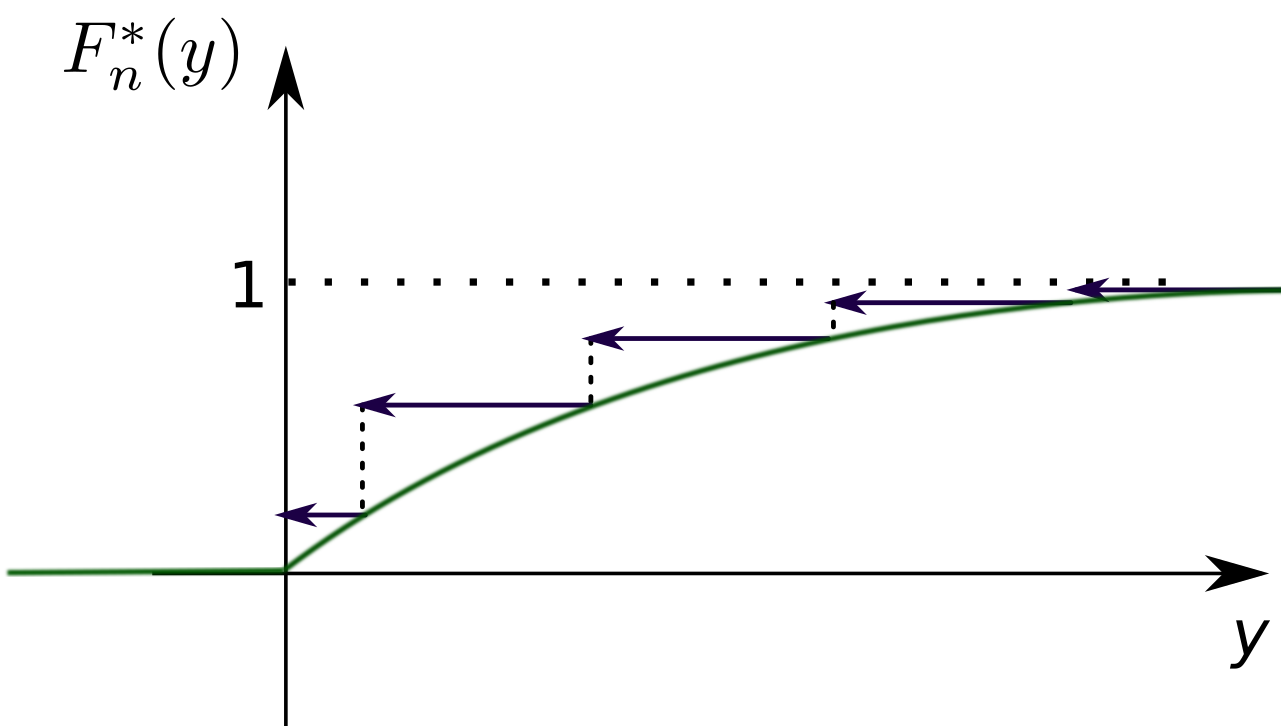
\includegraphics[width=0.5\textwidth]{assets/lectures_part_5-c8ce8645.png}
\end{wrapfigure}
\blue{Емпiричною функцією розподілу}, \\ побудованою за вибiркою $\xi_1, \dots , \xi_n$ об’єму $n$, називається випадкова
функцiя: \\$$F_n^* : \mathbb{R} \times \Sigma \to [0,1]$$ при кожному $y \in \mathbb{R}$ рiвна:
$$
F_y^* (y) = \frac{1}{n}  \sum\limits_{i = 1}^{ n}{ \index \left\lbrace \xi_i < y \right\rbrace}
$$
Із збільшенням кількості спостережень, емпірична функція розподілу наближається до теоретичної функції розподілу г.с. Зазначимо її основнi властивостi.

\begin{boxteo}[Консистентність]
Нехай $\xi_1, \dots , \xi_n$ – вибiрка з розподiлу $\mathcal{F}$ з ф.р. $F$ та нехай $F_n^*$ – емпiрична ф.р., яку
побудовано по цiй вибiрцi. Тодi, $\forall y \in \mathbb{R}:$
$$
F_n^* (y) \xrightarrow[n\to\infty]{\text{м.н.}} F(y)
$$
\end{boxteo}
\begin{spacing}{1}

\begin{proof}
За означенням:
$$
F_n^*(y) = \frac{1}{n}  \sum\limits_{i = 1}^{n}{\index (\xi_i < y)} \xrightarrow[n\to \infty]{\text{м.н.}} \underbrace{\mathbb{E} \index \left\lbrace \xi_i <y  \right\rbrace }_{=F_{\xi}(y)}
$$
Оскільки індикатори подій $\left\lbrace \xi_1 < y \right\rbrace, \left\lbrace \xi_1 < y \right\rbrace , \dots , \left\lbrace \xi_n < y \right\rbrace$ є незалежними й однаково розподiленими,
їх математичне сподiвання скiнчено:
$$
\mathbb{E} \index \left\lbrace \xi_1 < y \right\rbrace = 1 \cdot \mathbb{P} \left\lbrace \xi_1 < y \right\rbrace + 0 \cdot \mathbb{P} \left\lbrace \xi_1 \geq y \right\rbrace = \mathbb{P} \left\lbrace \xi_1 < y \right\rbrace = F(y)
$$
$$
\text{Застосовуючи посилений ЗВЧ}: \ \
F_n^* (y) = \frac{1}{n}  \sum\limits_{i = 1}^{n}{ \index \left\lbrace \xi_i <y \right\rbrace} \xrightarrow[n \to \infty]{\mathbb{P} } \mathbb{E}\index \left\lbrace \xi_1 < y \right\rbrace = F_{\xi}(y)
$$
\end{proof}
\end{spacing}
\begin{boxteo}[Глівенко-Кантеллі]
  В умовах теореми 3.1:
  $$
  \sup\limits_{y\in \mathbb{R}} \left| F_n^*(y) - F(y) \right| \xrightarrow[n \to \infty]{\text{м.н.}} 0
  $$
  Без доведення $\blacksquare$.
\end{boxteo}
\begin{boxteo}[Колмогорова]
  Нехай $\xi_1 , ..., \xi_n$ -- вибірка з неперервною ф.р.\\ $F \in C^1(\mathbb{R})$, а $F_n^*$ -- емпірична ф.р. \textbf{Тоді:}
  $$
  \sqrt{n}\sup\limits_{y\in \mathbb{R}} \left| F_n^*(y) - F(y) \right| \xrightarrow[n\to \infty]{}\eta,
  $$
  де в.в. $\eta$ має розподiл Колмогорова з неперервною ф.р.:
  $$
  F_{K} (y) = \begin{dcases}
    \sum\limits_{j = -\infty}^{ \infty}{ (-1)^j e^{-2j^2 y^2}}, & y \geq 0;\\
    0, & y < 0.
  \end{dcases}
  $$
  Без доведення $\blacksquare$.


\end{boxteo}



Нехай $\xi_1 , \dots, \xi_n$ --- вибірка з розподілу $\mathcal{F}$ з функцією розподілу $F$, а $F_n^*(y)$ -- емпірична функція розподілу. Тоді для довільного $y \in \mathbb{R}$:
\begin{enumerate}
	\item $\mathbb{E} F_n^* (y) = F(y)$ \ \ \textit{(незміщеність оцінки)};
	\item $\mathbb{D} F_n^* (y) = \dfrac{F(y) (1 -F(y))}{n} $;
	\item $\sqrt{ n} \left( F_n^* (y) - F(y) \right) \ \Longrightarrow \  N(0, F(y) (1 - F(y)))$ при $F(y) \neq 0,1$;
	\item величина $n F_n^* (y) $ має біноміальний розподіл $B(n. F(y))$.
\end{enumerate}
\begin{proof}
 Помітимо, що $\index \left\lbrace \xi_1 < y \right\rbrace$ має розподiл Бернуллi $B(F(y))$, а тому:
 $$
 \mathbb{E} \index \left\lbrace \xi_1 < y \right\rbrace = F(y) \qquad \quad \mathbb{D}\index \left\lbrace \xi_1 < y \right\rbrace = F(y) (1- F(y))
 $$
 Оскiльки, крiм того $\index \left\lbrace \xi_1 < y \right\rbrace, \index \left\lbrace \xi_2 < y \right\rbrace, \dots $ є незалежними, то:
 $$
 nF_n^*(y) =  \sum\limits_{i = 1}^{n}{\index \left\lbrace \xi_1 \right\rbrace} \ \sim \  B(n, F(y)) \ \Longrightarrow \ \textit{(властивість 4)}
 $$
 Властивостi 1, 2 випливають з 4-ї.
 Для доведення 3-ї використаємо ЦГТ:
 $$
 \sqrt{n} (F_n^* - F(y)) = \frac{ \sum\limits_{i = 1}^{n}{\index \left\lbrace \xi_i < y \right\rbrace - nF(y)}}{\sqrt{n}} =\frac{ \sum\limits_{i = 1}^{n}{\index \left\lbrace \xi_i < y \right\rbrace - n \mathbb{E} \index (\xi_1 < y)}}{\sqrt{n} } \  \Longrightarrow
 $$
 $$
 \Longrightarrow \  N(0, \mathbb{D} \index \left\lbrace  \xi_1 < y \right\rbrace ) = N(0, F(y)(1 - F(y))) \ \  n \to \infty.
 $$
\end{proof}
\subsection{Властивостi вибiркових моментiв.}
Нехай $\xi_1 , \dots , \xi_n$ --- вибірка з розподілу $\mathcal{F}$. Тоді:

\begin{enumerate}
	\item Якщо $\mathbb{E} |\xi_1| < \infty $, то $\mathbb{E} \overline{\xi} = \mathbb{E} \xi_1 = a$ -- незміщеність $\overline{\xi}$;
	\item Якщо $\mathbb{E} |\xi_1| < \infty $, то $\overline{\xi} \xrightarrow[n\to\infty]{\mathbb{P}} \mathbb{E} \xi_1 = a$ -- консистентність $\overline{\xi}$;
	\item Якщо $\mathbb{D} \xi_1 < \infty, \mathbb{D} \xi_1 \neq 0$, то $\sqrt{n} (\overline{\xi} - \mathbb{E} \xi_1) \xrightarrow[n\to\infty]{} N(0, \mathbb{D} \xi_1)$
\end{enumerate}
\begin{proof}\ \\
 \begin{itemize}
 	\item Властивiсть 1 випливає iз властивостей математичного сподiвання.\\
	\item Доведення 2 та 3 випливає безпосередньо iз застосування ЗВЧ Хiнчина та ЦГТ,
вiдповiдно.
 \end{itemize}
\end{proof}
\newpage
Вибiрковий $k$-й момент $\overline{\xi}^k$  є незмiщенною, консистентною та асимптотично нормальною для
теоретичного $k$-го момента.
Нехай $\xi_1 , \dots, \xi_n$ – вибiрка з розподiлу $\mathcal{F}$. Тодi:
\begin{enumerate}
	\item Якщо $\mathbb{E} |\xi_1|^k < \infty , \mathbb{E} \overline{\xi}^k = \mathbb{E} \xi_1^k = m_k ;$
	\item  Якщо $\mathbb{E} |\xi_1|^k < \infty$ , то $ \overline{\xi}^k \xrightarrow[n\to\infty]{\mathbb{P}} \mathbb{E} \xi_1^k;$
	\item Якщо $\mathbb{D}\xi_1^k < \infty , \mathbb{D} \xi_1^k \neq 0$, то $\sqrt{n} (\overline{\xi}^k - \mathbb{E} \xi_1^k) \xrightarrow[n\to\infty]{} N(0, \mathbb{D} \xi_1^k)$
\end{enumerate}
Вибiрковi дисперсiї мають наступнi властивостi:\par
Нехай $\xi_1 , \dots , \xi_n$ --- вибірка з розподілу $\mathcal{F}$ та $\mathbb{D} \xi_1 < \infty$. Тодi:
\begin{enumerate}
	\item $\mathbb{E} s^2 = \frac{n-1}{n} \mathbb{D}\xi_1 = \frac{n-1}{n}\sigma^2 \neq \sigma^2 , \mathbb{E}s^2_0 = \mathbb{D} \xi_1 = \sigma^2  $;
	\item $s^2 \xrightarrow[n\to\infty]{\mathbb{P}} \mathbb{D} \xi_1 = \sigma^2 , s^2_0 \xrightarrow[n\to\infty]{\mathbb{P}} \mathbb{D}\xi_1 = \sigma^2 $;

\end{enumerate}
\newpage
\section{Точкові оцінки параметрів Г.С.}
\vspace*{-2em}
Нехай є генеральна сукупнісь $\mathcal{F}$ випадкової величини $\xi$ з відомим розподілом, але невідомим вектором параметрів $\overrightarrow{\theta} = \begin{bmatrix}
 \theta_1 & \cdots & \theta_n
\end{bmatrix}$.\\
\red{Оцінка $\theta^*$}  параметру $\theta$ --- деяка статистика, значення  якої ''близькі'' до $\theta$:
$$
\theta_n^* = \varphi(\xi_1 , \dots, \xi_n) \qquad \quad \theta \approx \theta^* (\xi_1 , ... , \xi_n)
$$
\vspace*{-4.5em}
\subsection{Методи побудови точкових оцінок.}
\vspace*{-1em}
\subsubsection{Метод моментів.}
\vspace*{-1em}
Нехай є генеральна сукупнісь $\mathcal{F}$ випадкової величини $\xi$, яка має характеристики:\\
{\centering
	\blue{Теоретичні } ($\mathbb{E}\xi, \mathbb{D}\xi, \mathbb{E} \xi^k , \dots$)
	\ та \
	 \blue{Вибіркові } ($\overline{\xi}, \mathbb{D}^{*, **,***}_\xi$)\\
}
Ідея методу моментів -- прийняти вибіркові значення характеристик за теоретичні.
\vspace*{-1.5em}
\subsubsection{Метод максимальної вірогідності (MLE).}
\vspace*{-1em}
Нехай $\mathcal{F}$ -- дискретна генеральна сукупність. Маємо:
$
\xi_1 , \dots , \xi_n \xrightarrow{\text{реалізація}} x_1 , \dots , x_n
$.
$$
\mathcal{L} (x_1, \dots, x_n, \theta) = \mathbb{P} \left\lbrace \xi_1 = x_1 , \dots , \xi_n = x_n \right\rbrace \  - \  \red{ Likelihood function.}
$$
\vspace*{-1em}
$$
\mathcal{L} (x_1, \dots, x_n, \theta)  = \left| \independent \right| =  \prod\limits_{i = 1}^{n}{ \mathbb{P} \left\lbrace \xi_i = x_i \right\rbrace} =
 \prod\limits_{i = 1}^{ \infty}{\mathbb{P}_{\theta} \left\lbrace \xi= x_i \right\rbrace} \xrightarrow{\theta} \max
$$
Надалі максимізуємо вираз, застосувавши властивість монотонності логарифма:
\vspace*{-0.5em}
$$
\ln \mathcal{L} (x_1, \dots, x_n, \theta)   =  \sum\limits_{i = 1}^{ \infty} { \ln \mathbb{P}_{\theta} \left\lbrace \xi= x_i \right\rbrace} \xrightarrow{\theta} \max
$$
\vspace*{-0.5em}
$$
\frac{ \d \ln \mathcal{L} (x_1, \dots, x_n, \theta)}{\d \theta}    =
 \sum\limits_{i = 1}^{ \infty} { \frac{\d }{\d \theta}  \ln \mathbb{P}_{\theta} \left\lbrace \xi= x_i \right\rbrace} =  0 \ \Longrightarrow \  \theta^*
$$
Нехай $\mathcal{F}$ -- неперервна генеральна сукупність. Маємо щільність розподілу вибірки:
\vspace*{-0.5em}
$$
\mathcal{L} (x_1, \dots, x_n , \theta) = f_{\xi_1 , \dots , \xi_n }(x_1, x_2 , \dots, x_n) = |\independent| =  \prod\limits_{i = 1}^{n}{ f_{\xi_i} (x_i)} = \prod\limits_{i = 1}^{n}{ f_{\xi} (x_i)}
$$
Скористалися однаковою розподіленістю величин $\xi_1 , \dots , \xi_n$ з щільністю $f_{\xi} (x)$.\\ Надалі пошук оцінки $\theta^*$ аналогічно до дискретного випадку.
\subsection{Властивості оцінок.}
\subsubsection{Незміщеність(unbiasedness).}
\begin{defo}$\theta^*$ --- \red{незміщенна} оцінка параметру $\theta$, якщо $\mathbb{E} \theta^* = \theta$.
\end{defo}
\begin{defo}$\theta^*_n$ --- \red{ асимптотично незміщенна} оцінка параметру $\theta$, якщо:
$$\mathbb{E} \theta^* \xrightarrow[n\to\infty]{} \theta$$
\end{defo}
\subsubsection{Консистентність.}
\begin{defo} $\theta^*_n$ називається \red{консистентною} оцінкою параметра $\theta$, якщо:
$$
\theta^*_n \xrightarrow[n\to\infty]{\mathbb{P}} \theta \quad \blue{--- слабка} \qquad \quad
\theta^*_n \xrightarrow[n\to\infty]{\text{м.н.}} \theta \quad \blue{--- сильна }
$$
\end{defo}
\textit{Як перевіряти консистентність?}
\begin{enumerate}
	\item За (посиленим, якщо у сенсі \textit{м.н.}) законом великих чисел.
	\item За означенням збіжності ($\mathbb{P}$, \textit{м.н.}).
	\item \textbf{Лема.} Для $\theta^*_n$: $\begin{cases}
	 \text{(Асимптотично) незміщена.}\\
	 \text{} \mathbb{D}\theta_n^* \xrightarrow[n\to\infty]{} 0
	\end{cases} \Longrightarrow \theta_n^*$ -- слабко консистентна.
	\begin{proof}
$$
\begin{cases}
 \mathbb{E}  \theta_n^* \xrightarrow[n\to\infty]{} 0;\\
 \mathbb{D} \theta_n^* \xrightarrow[n\to\infty]{} 0.
\end{cases}
\Longrightarrow \left| \begin{gathered}
\text{За критерієм}\\
\mathbb{L}_2 \text{-збіжності до } const
\end{gathered} \right| \Longrightarrow \theta_n^* \xrightarrow[n\to\infty]{\mathbb{L}_2} \theta \Longrightarrow \theta_n^* \xrightarrow[n\to\infty]{\mathbb{P}} \theta
$$
	\end{proof}
\end{enumerate}


\end{document}
